\chapter{Concept and Design}
\label{cha:conceptanddesign}

\textbf{We need to describe here what do we want to achieve, what do we mean by modelling and visualizing macroscopic movements etc - thus general architecture that we have 3 components, Stop Detection from telekom data based on movements and updates of "areas" in your mobile phone, Clustering of Stops to find most popular "stops" in the city, Graph Generation to find where do the people move and in what amount
}
\section{Stop Location Detection}

\subsection{Stop Detection for proactive localization based services}

Analyzing different approaches for stop detection based on localization data (ref. \autoref{cha:introduction_appr_stopdet}), we decided to design algorithm based on human behavior regarding mobility within the cities (ref. \autoref{cha:introduction_hummob}) and reusing the concept of Mobility Index (ref. \autoref{cha:introduction_mob_index_sect})). Stop Location Detection Algorithm have to be able not only identify the time of start stop, but also the stop location.

\subsection{Mobility index based approach}

In related works about mobility index discussed in \autoref{cha:introduction_mob_index_sect}, the approach to stop detection using mobility index is bound to the way the data is being sampled (handover from one GSM cell to another). The data is recorded whenever mobile device changes its GSM cell. 
\\\\
In case of the approach discussed in this paper (\autoref{cha:introduction_methodo}), the situation is similar, however instead of GSM cells we have artificially created area around the location, and while new location is obtained at some distance after movement, new area might need to be updated and points is being recorded.
\\\\
In a populated area, the user can move from one area to another after several seconds or only after minutes. Thus, if within a certain
period of time (called mobility index time window) the user stays in the same area (mobility index is equal to 0) or changes the areas with small pace (mobility index is below certain threshold) it can be assumed that the user is immobile or having short stay at the location somewhere within that time window. 
\\\\
Approach based on mobility index could precisely identify how mobile has been user within the certain time period and identify longer stop locations, however mobility index is not able to identify short stops at location where in the certain time window user been moving fast, stopped and moving fast again. 

\subsection{Human Behavior based approach}

This approach targets the condition for movement between two points, which has to be satisfied, so that it can be considered as a stay within the certain distance. 
\\\\
The \autoref{cha:introduction_hummob} discusses, that in average, walking human is covering a short distances with the speed of 4km/h. However for movement on long distances, user will most likely use city or private transport, and thus his speed can vary much in that time/distance period.
\\\\
This means that stop detection based on speed of movement over long distance might not be effective, however, on small distances it might quite precisely identify short stays at certain locations, in between high mobility of the user.  

\section{Clustering of Stops}

Clustering can be described as "\textit{the task of grouping a set of objects in such a way that objects in the same group (called a cluster) are more similar (in some sense or another) to each other than to those in other groups (clusters)}" \cite{clustering}. 
\\\\
After our stop detection algorithm has detected the proper stops we want to perform some analysis on these. Our goal is to get the overall movement patterns of the population of a certain area, which means we are interested in \textbf{macroscopic} movements and not microscopic (individual) movement. If we would consider every individual our analysis algorithms would get fed with a lot of noise (outliers) which would make our data mining and prediction difficult and inaccurate. Meaning, \textit{Macroscopic Movements} are not interesting in tracking individuals but rather seeing the big picture.

 Once our clustering algorithm has been applied, and we have the overall picture, we can see which stops are most popular, where people are moving from them, and how long they stay at a certain location. One could then perform some interesting graph analysis on these locations, answering questions such as "what is the probability that a person moves from point \textit{A} to \textit{B}?", or "what is the average stop time at location \textit{A}?". 
 
 To achieve these clusters, which represents our interesting stop locations, we need to apply some clustering algorithm. There are different types of clustering (such as centroid, distribution, or density-based), and different algorithms with parameters that can be applied (such as K-means, DBScan, or OPTICS). However, they all work to achieve the same goal of structuring (clustering, grouping) similar objects and neglecting outliers from these groups. The algorithm and parameters are application sensitive and our choice will be handled in the \textit{evaluation} section.

\begin{figure}[!ht]
	\centering
	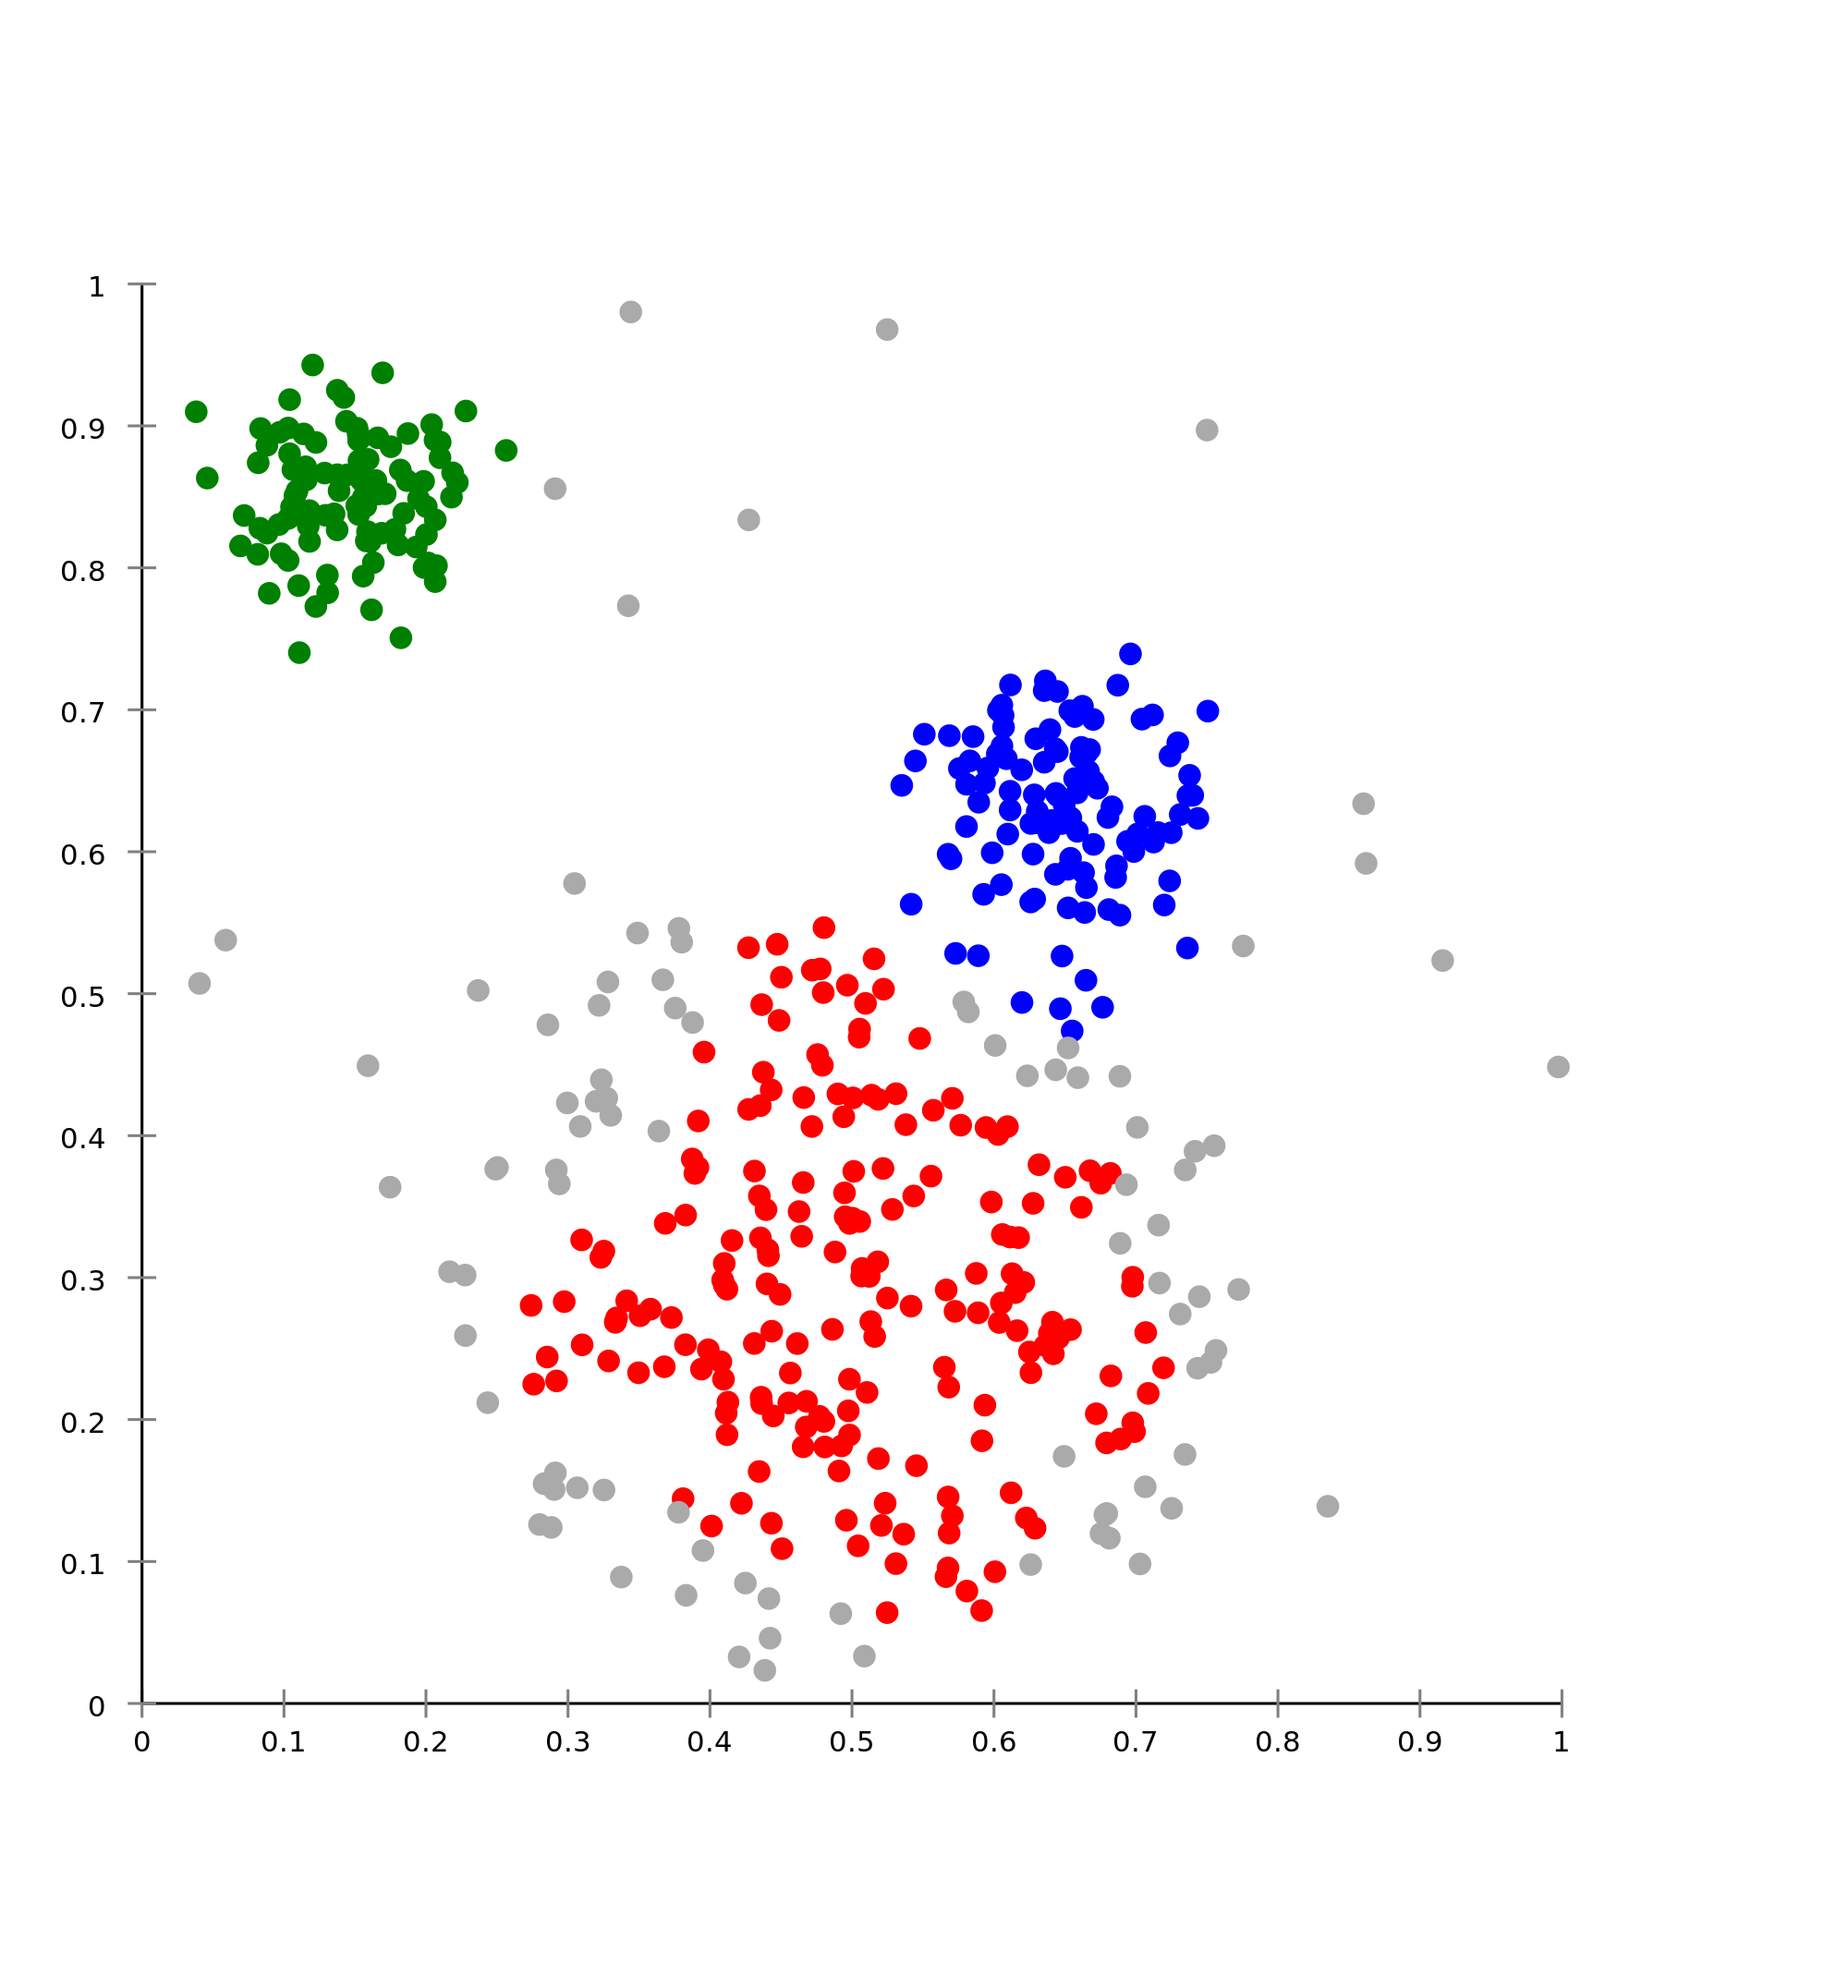
\includegraphics[width=0.6\textwidth]{images/clustering.png}
	\caption{ Clustering applied to a dataset. }
	\label{fig:clustering}
\end{figure} 



\FloatBarrier
\section{City Movements Graph}

\FloatBarrier